
\chapter{Instrumentation documents}

Every technical discipline has its own standardized way(s) of making descriptive diagrams, and instrumentation is no exception.  The scope of instrumentation is so broad, however, that no one form of diagram is sufficient to capture all we might need to represent.  This chapter will discuss three different types of instrumentation diagrams:

\begin{itemize}
\item Process Flow Diagrams (PFDs)
\item Process and Instrument diagrams (P\&IDs)
\item Loop diagrams (``loop sheets'')
\item Functional diagrams
\end{itemize}

At the highest level, the instrument technician is interested in the interconnections of process vessels, pipes, and flow paths of process fluids.  The proper form of diagram to represent the ``big picture'' of a process is called a \textit{process flow diagram}.  Individual instruments are sparsely represented in a PFD, because the focus of the diagram is the process itself.

At the lowest level, the instrument technician is interested in the interconnections of individual instruments, including all the wire numbers, terminal numbers, cable types, instrument calibration ranges, etc.  The proper form of diagram for this level of fine detail is called a \textit{loop diagram}.  Here, the process vessels and piping are sparsely represented, because the focus of the diagram is the instruments themselves.

\textit{Process and instrument diagrams} (P\&IDs) lie somewhere in the middle between process flow diagrams and loop diagrams.  A P\&ID shows the layout of all relevant process vessels, pipes, and machinery, but with instruments superimposed on the diagram showing what gets measured and what gets controlled.  Here, one can view the flow of the process as well as the ``flow'' of information between instruments measuring and controlling the process.

\textit{Functional} diagrams are used for an entirely different purpose: to document the \textit{strategy} of a control system.  In a functional diagram, emphasis is placed on the algorithms used to control a process, as opposed to piping, wiring, or instrument connections.  These diagrams are commonly found within the power generation industry, but are sometimes used in other industries as well.

\vskip 10pt

An instrument technician must often switch between different diagrams when troubleshooting a complex control system.  There is simply too much detail for any one diagram to show everything.  Even if the page were large enough, a ``show everything'' diagram would be so turgid with details that it would be difficult to focus on any particular grouping of details you happened to be interested in.  The narrowing of scope with the progression from PFD to loop diagram may be visualized as a process of ``zooming in,'' as though one were viewing a process through the lens of a microscope at different powers.  First you begin with a PFD or P\&ID to get an overview of the process, to see how the major components interact.  Then, once you have identified which instrument ``loop'' you need to investigate, you go to the appropriate loop diagram to see the interconnection details of that instrument system so you know where to connect your test equipment and what signals you expect to find when you do.

Another analogy for this progression of documents is a map, or more precisely, a globe, an atlas, and a city street map.  The globe gives you the ``big picture'' of the Earth, countries, and major cities.  An atlas allows you to ``zoom in'' to see details of particular provinces, states, and principalities, and the routes of travel connecting them all.  A city map shows you major and minor roads, canals, alleyways, and perhaps even some addresses in order for you to find your way to a particular destination.  It would be impractical to have a globe large enough to show you all the details of every city!  Furthermore, a globe comprehensive enough to show you all these details would have to be updated \textit{very} frequently to keep up with all cities' road changes.  There is a certain economy inherent to the omission of fine details, both in ease of use and in ease of maintenance.










\filbreak
\section{Process Flow Diagrams}

To show a practical process example, let's examine three diagrams for a compressor control system, beginning with a Process Flow Diagram, or PFD.  In this fictitious process, water is being evaporated from a process solution under partial vacuum (provided by the compressor).  The compressor then transports the vapors to a ``knockout drum'' where they condense into liquid form.  As a typical PFD, this diagram shows the major interconnections of process vessels and equipment, but omits details such as instrument signal lines and auxiliary instruments:  \index{Process Flow Diagram (PFD)}  \index{PFD}

$$\includegraphics{intro_11.eps}$$

One might guess the instrument interconnections based on the instruments' labels.  For instance, a good guess would be that the level transmitter (LT) on the bottom of the knockout drum might send the signal that eventually controls the level valve (LV) on the bottom of that same vessel.  One might also guess that the temperature transmitter (TT) on the top of the evaporator might be part of the temperature control system that lets steam into the heating jacket of that vessel.

Based on this diagram alone, one would be hard-pressed to determine what control system, if any, controls the compressor itself.  All the PFD shows relating directly to the compressor is a flow transmitter (FT) on the suction line.  This level of uncertainty is perfectly acceptable for a PFD, because its purpose is merely to show the general flow of the process itself, and only a bare minimum of control instrumentation.




\filbreak
\section{Process and Instrument Diagrams}

The next level of detail is the Process and Instrument Diagram\footnote{Sometimes P\&ID stands for \textit{Piping} and Instrument Diagram.  Either way, it means the same thing.}, or P\&ID.  Here, we see a ``zooming in'' of scope from the whole evaporator process to the compressor as a unit.  The evaporator and knockout vessels almost fade into the background, with their associated instruments absent from view\footnote{It should be noted that the ``zooming in'' of scope in a P\&ID does not necessarily mean the scope of other areas of the process must be ``zoomed out.''  In fact, it is rather typical in a P\&ID that the \textit{entire} process system is shown in finer detail than in a PFD, but not all on one page.  In other words, while a PFD may depict a process in its entirely on one piece of paper, a comprehensive P\&ID will typically span multiple pieces of paper, each one detailing a section of the process system.}:  \index{Process and Instrument Diagram (P\&ID)}  \index{P\&ID}  \index{Piping and Instrument Diagram (P\&ID)} 

$$\includegraphics{intro_12.eps}$$

Now we see there is more instrumentation associated with the compressor than just a flow transmitter.  There is also a differential pressure transmitter (PDT), a flow indicating controller (FIC), and a ``recycle'' control valve allowing some of the vapor coming out of the compressor's discharge line to go back around into the compressor's suction line.  Additionally, we have a pair of temperature transmitters reporting suction and discharge line temperatures to an indicating recorder.

Some other noteworthy details emerge in the P\&ID as well.  We see that the flow transmitter, flow controller, pressure transmitter, and flow valve all bear a common number: 42.  This common ``loop number'' indicates these four instruments are all part of the same control system.  An instrument with any other loop number is part of a different control system, measuring and/or controlling some other function in the process.  Examples of this include the two temperature transmitters and their respective recorders, bearing the loop numbers 41 and 43.

Please note the differences in the instrument ``bubbles'' as shown on this P\&ID.  Some of the bubbles are just open circles, where others have lines going through the middle.  Each of these symbols has meaning according to the ISA (Instrumentation, Systems, and Automation society) standard:

$$\includegraphics{intro_13.eps}$$

The type of ``bubble'' used for each instrument tells us something about its location.  This, obviously, is quite important when working in a facility with many thousands of instruments scattered over acres of facility area, structures, and buildings.

The rectangular box enclosing both temperature recorders shows they are part of the same physical instrument.  In other words, this indicates there is really only one temperature recorder instrument, and that it plots both suction and discharge temperatures (most likely on the same trend graph).  This suggests that each bubble may not necessarily represent a discrete, physical instrument, but rather an instrument \textit{function} that may reside in a multi-function device.

Details we do not see on this P\&ID include cable types, wire numbers, terminal blocks, junction boxes, instrument calibration ranges, failure modes, power sources, and the like.  To examine this level of detail, we must turn to another document called a \textit{loop diagram}.










\filbreak
\section{Loop diagrams}

Finally, we arrive at the loop diagram (sometimes called a \textit{loop sheet}) for the compressor surge control system (loop number 42):  \index{Loop diagram}  \index{Loop sheet}

$$\includegraphics{intro_09.eps}$$

Here we see that the P\&ID didn't show us all the instruments in this control ``loop.''  Not only do we have two transmitters, a controller, and a valve; we also have two signal transducers.  Transducer 42a modifies the flow transmitter's signal before it goes into the controller, and transducer 42b converts the electronic 4 to 20 mA signal into a pneumatic 3 to 15 PSI air pressure signal.  Each instrument ``bubble'' in a loop diagram represents an individual device, with its own terminals for connecting wires.

Note that dashed lines now represent individual copper wires instead of whole cables.  Electrical terminals where these wires connect to are represented by squares with numbers in them.  Fluid ports on instruments are also represented by labeled squares.  Cable numbers, wire colors, junction block numbers, panel identification, and even grounding points are all shown in loop diagrams.  The only type of diagram for this system more detailed than a loop diagram would be an electronic schematic diagram for an individual instrument, which of course would only show details pertaining to that one instrument.  Thus, the loop diagram is the most detailed form of diagram for a control system as a whole, and as such it must contain all details omitted by PFDs and P\&IDs alike.

To the novice it may seem excessive to include such trivia as wire colors in a loop diagram.  To the experienced instrument technician who has had to work on systems lacking such documented detail, this information is highly valued.  The more detail you put into a loop diagram, the easier it makes the inevitable job of maintaining that system at some later date.  When a loop diagram shows you exactly what wire color to expect at exactly what point in an instrumentation system, and exactly what terminal that wire should connect to, it becomes much easier to proceed with any troubleshooting, calibration, or upgrade task.

\vskip 10pt

Loop diagrams are fairly constrained in their layout as per the ISA 5.1 standard.  Field instruments are always placed on the left-hand side, while control-panel or control-room instruments must be located on the right-hand side.  Text describing instrument tags, ranges, and notes are always placed on the bottom.  Unlike PFDs and P\&IDs where component layout is largely left to the whim of the designer drawing the diagram, loop sheets offer little room for creativity.  This is intentional, as creativity and readability are mutually exclusive in cases where there is an immense amount of technical detail embedded in a diagram.  It is simply easier to find details you're looking for when you know \textit{exactly} where they ought to be.

\vskip 10pt

An interesting detail seen on this loop diagram is an entry specifying ``input calibration'' and ``output calibration'' for each and every instrument in the system.  This is actually a very important concept to keep in mind when troubleshooting a complex instrumentation system: every instrument has at least one input and at least one output, with some sort of mathematical relationship between the two.  Diagnosing where a problem lies within a measurement or control system often means testing various instruments to see if their output responses appropriately match their input conditions, so it is important to document these input and output ranges.

For example, one way to test the flow transmitter in this system would be to subject it to a number of different pressures within its range (specified in the diagram as 0 to 100 inches of water column differential) and seeing whether or not the current signal output by the transmitter was consistently proportional to the applied pressure (e.g. 4 mA at 0 inches pressure, 20 mA at 100 inches pressure, 12 mA at 50 inches pressure, etc.).

Given the fact that a calibration error or malfunction in any one of these instruments can cause a problem for the control system as a whole, it is nice to know there is a way to determine which instrument is to blame and which instruments are not.  This general principle holds true regardless of the instrument's type or technology.  You can use the same input-versus-output test procedure to verify the proper operation of a pneumatic (3 to 15 PSI) level transmitter or an analog electronic (4 to 20 mA) flow transmitter or a digital (fieldbus) temperature transmitter alike.  Each and every instrument has an input and an output, and there is always a predictable (and testable) correlation from one to the other.

\vskip 10pt

\filbreak

Another interesting detail seen on this loop diagram is the \textit{direction of action} of each instrument.  You will notice a box and arrow (pointing either up or down) next to each instrument bubble.  An ``up'' arrow ($\uparrow$) represents a \textit{direct-acting} instrument: one whose output signal increases as the input stimulus increases.  A ``down'' arrow ($\downarrow$) represents a \textit{reverse-acting} instrument: one whose output signal decreases as the input stimulus increases.  All the instruments in this loop are direct-acting with the exception of the pressure differential transmitter PDT-42: \index{Direct-acting transmitter}  \index{Reverse-acting transmitter}

$$
\includegraphics{intro_18.eps}$$

Here, the ``down'' arrow tells us the transmitter will output a full-range signal (20 mA) when it senses zero differential pressure, and a 0\% signal (4 mA) when sensing a full 200 PSI differential.  While this calibration may seem confusing and unwarranted, it serves a definite purpose in this particular control system.  Since the transmitter's current signal decreases as pressure increases, and the controller must be correspondingly configured, a decreasing current signal will be interpreted by the controller as a high differential pressure.  If any wire connection fails in the 4-20 mA current loop for that transmitter, the resulting 0 mA signal will be naturally ``seen'' by the controller as a pressure over-range condition.  Excessive pressure drop across a compressor is considered dangerous because it may lead to the compressor surging\footnote{Compressor ``surge'' is a violent and potentially self-destructing action experienced by a centrifugal compressor if the pressure drop across it becomes too high and the flow rate through it becomes too low.  Surging may be prevented by opening up a ``recycle'' valve from the compressor's discharge line to the suction line, ensuring adequate flow through the compressor while simultaneously unloading the high pressure differential across it.}.  Thus, the controller will naturally take action to prevent surge by commanding the anti-surge control valve to open, because it ``thinks'' the compressor is about to surge.  In other words, the transmitter is intentionally calibrated to be reverse-acting such that any break in the signal wiring will naturally bring the system to its safest condition.








\filbreak
\section{Functional diagrams}

A unique form of technical diagram for describing the abstract functions comprising a control system (e.g. PID controllers, rate limiters, manual loaders) is a \textit{functional diagram}\footnote{Functional diagrams are sometimes referred to as \textit{SAMA} diagrams in honor of the organization responsible for their standardization, the \textit{Scientific Apparatus Makers Association}.  This organization has been succeeded by the Measurement, Control, and Automation Association (MCAA), thus obsoleting the ``SAMA'' acronym.}.  This form of document finds wide application in the power generation industry to document control strategies.  Functional diagrams focus on the flow of information within a control system rather than on the process piping or instrument interconnections (wires, tubes, etc.).  The general flow of a functional diagram is top-to-bottom, with the process sensing instrument (transmitter) located at the top and the final control element (valve or variable-speed motor) located at the bottom.  No attempt is made to arrange symbols in a functional diagram to correspond with actual equipment layout: these diagrams are all about the \textit{algorithms} used to make control decisions, and nothing more. \index{Functional diagram}  \index{SAMA diagram} \index{Algorithm, control}

A sample functional diagram appears here, showing a flow transmitter (FT) sending a process variable signal to a PID controller, which then sends a manipulated variable signal to a flow control valve (FCV):

$$\includegraphics{intro_14.eps}$$

\filbreak

A cascaded control system, where the output of one controller acts as the setpoint for another controller to follow, appears in functional diagram form like this:

$$\includegraphics{intro_15.eps}$$

In this case, the primary controller senses the level in a vessel, commanding the secondary (flow) controller to maintain the necessary amount of flow either in or out of the vessel as needed to maintain level at some setpoint.

\filbreak

Functional diagrams may show varying degrees of detail about the control strategies they document.  For example, you may see the auto/manual controls represented as separate entities in a functional diagram, apart from the basic PID controller function.  In the following example, we see a transfer block (T) and two manual adjustment blocks (A) providing a human operator the ability to separately adjust the controller's setpoint and output (manipulated) variables, and to transfer between automatic and manual modes:

$$\includegraphics{intro_16.eps}$$

\filbreak

Rectangular blocks such as the $\Delta$, P, I, and D shown in this diagram represent automatic functions.  Diamond-shaped blocks such as the A and T blocks are manual functions (i.e. set by a human operator).  Showing even more detail, the following functional diagram indicates the presence of \textit{setpoint tracking} in the controller algorithm, a feature that forces the setpoint value to equal the process variable value any time the controller is in manual mode: \index{Setpoint tracking}

$$\includegraphics{intro_17.eps}$$

Here we see a new type of line: dashed instead of solid.  This too has meaning in the world of functional diagrams.  Solid lines represent analog (continuously variable) signals such as process variable, setpoint, and manipulated variable.  Dashed lines represent discrete (on/off) signal paths, in this case the auto/manual state of the controller commanding the PID algorithm to get its setpoint either from the operator's input (A) or from the process variable input (the flow transmitter: FT).









\filbreak
\section{Instrument and process equipment symbols} 

Standarder som skal legges inn her. 
%\begin{itemize}[noitemsep]
%	\item NS-EN ISO 10628-1:2015 Diagrammer for kjemisk og petrokjemisk industri - Del 1: Spesifikasjon av diagrammer (ISO 10628-1:2014)
%	\item NS-EN ISO 10628-2:2012 Diagrammer for kjemisk og petrokjemisk industri - Del 2: Grafiske symboler 
%\end{itemize}



This section shows some of the many instrument symbols found in different types of technical diagrams used to document instrument systems.

\filbreak
\subsection{Line types}

$$\includegraphics{diagrams00.eps}$$

Note: the single backslash signifying a ``discrete'' or ``binary'' signal type has been removed from the ISA standard as of the 2009 ANSI publication.  Regular pneumatic and electrical line symbols may represent either continuous or discrete states.  The ``triple-slash'' alternative linetype for electrical symbols is also absent from the 2009 ANSI/ISA standard.

\filbreak
\subsection{Process/Instrument line connections}

$$\includegraphics{diagrams04.eps}$$


\filbreak
\subsection{Instrument bubbles}

$$\includegraphics{diagrams01.eps}$$



\filbreak
\subsection{Process valve types}

$$\includegraphics{diagrams02.eps}$$



\filbreak
\subsection{Valve actuator types}

$$\includegraphics{diagrams03.eps}$$



\filbreak
\subsection{Valve failure mode}

$$\includegraphics{diagrams05.eps}$$



\filbreak
\subsection{Liquid level measurement devices}

$$\includegraphics{diagrams13.eps}$$



\filbreak
\subsection{Flow measurement devices (flowing left-to-right)}

$$\includegraphics{diagrams06.eps}$$

\filbreak

$$\includegraphics{diagrams14.eps}$$



\filbreak
\subsection{Process equipment}

$$\includegraphics{diagrams07.eps}$$



\filbreak
\subsection{Functional diagram symbols}

$$\includegraphics{diagrams08.eps}$$




\filbreak
\subsection{Single-line electrical diagram symbols}

$$\includegraphics{diagrams09.eps}$$

\filbreak

$$\includegraphics{diagrams10.eps}$$



\filbreak
\subsection{Fluid power diagram symbols}

$$\includegraphics{diagrams11.eps}$$

\filbreak

$$\includegraphics{diagrams12.eps}$$




\filbreak
\section{Instrument identifiserings tag} 

Frem til nå har vi sett på flere typer instrument skjema, i alle har de for skjellige instrumentene hatt en kode som forklarer funksjonen. TT er en Termperatur Transmitter, PDT er en Trykk Differanse Transmitter eller FV er en Flow Ventil. Disse bokstavene er definert i ISO 14617-6. 

Hvert instrument i et automatisert anlegg bør ha sin egen unike \textit{tag}, bestående av en bokstavkode som beskriver instrumentet sin funksjon i tillegg til et tall som beskriver hvilken sløyfe det tilhører. Det kan også være nummer som referer til et større om område i anlegget. Det samme instrumentet kan brukes flere plasser i en sløyfe, en kan da bruke en bokstavkode til de ulike delene.  

Som et eksempel, hvis vi ser et instrument med tag\texttt{FC-135}, så vet vi at det er en \textit{flow controller} (FC) for sløyfe 135. I et stort prosessanlegg med flere områder med ulike funksjoner, ville kanskje dette instrumentet vært merket 12-FC-135 (flow controller for sløyfe 135 i område 12. ) Om denne støyfen inneholdt flere regulatorer (controllere), kunne skilt mellom dem ved å bruke etterfølgende bokstaver på sløyfenummeret. (12-FC-135A, 12-FC-135B, 12-FC-135C). 

Alle instrumenter i en sløyfe blir identifisert med en bokstav som beskriver variabelen som sløyfen skal regulere, helt uavhengig av den fysike oppbygning av instrumentet. Vår tenkte flow controller FC-135, kan være fysisk lik nivå regulatoren i sløyfe \#72 (LC-72), eller til temperatur regulatoren i sløyfe \#288 (TC-288). Det som gjør FC-135 til en strømningsregulator er at den primære variabelen den skal regulere er strømning. Alle andre instrumenter i denne sløyfen vil også ha F som første bokstav\footnote{Exceptions do exist to this rule.  For example, in a cascade or feedforward loop where multiple transmitters feed into one or more controllers, each transmitter is identified by the type of process variable \textit{it} senses, and each controller's identifying tag follows suit.}. I en nivåreguleringssøyfe kan dette se slik ut: Transmitteren merkes "LT" selv om den måler trykk for å angi nivå, regulatoren merkes "LC" og reguleringsventilen merkes LV selv om den i prakses justerer strømning. Dette fordi deres primære funksjon er å bidra til nivåregulering. 

\filbreak

Bokstaver som kan brukes til å identifisere instrumenter angis i standarder. ISO14617-6 er en slik standard. Det finnes flere standarder i bruker rundt om i verden og gamle anlegg kan være basert på eldre standarder. Tabellen nedenfor er et utdrag av vanlige bokstaver som brukes. Legg merke til at bruken av signalomformer definerer en unik variabel. f.eks. en "PT" er en trykktransmitter som måler trykk på en plass, mens "PDT" er en måling av trykkdifferanse mellom to punkter. På samme måte kan "TC" være en temperaturregulator som regulerer temperaturen i en prosess, mens "TKC" er en regulator som regulerer temperatur forandring. 

% No blank lines allowed between lines of an \halign structure!
% I use comments (%) instead, so that TeX doesn't choke.
\begin{center}
\begin{tabular}{ | m{1.5cm} | m{4.5cm}| m{4.5cm} | m{4.5cm} |} 
\hline
\multicolumn{4}{|c|}{Bokstavkode for indentifisering av instrumentfunksjoner} \\
\hline
	Bokstav & Variabel& Signalomformer & Funksjon \\ 
\hline
	A&&&Alarm\\
\hline
	B&&&Visning av diskre status\\
\hline
	C&&&Regulerende\\
\hline
	D&Densitet&Differanse&\\
\hline
	E&Elektrisk variabel&&Elemens (følende)\\
\hline
	F&Flow rate&Forhold&\\
\hline
	G&Posisjon, lengde&&Visning\\
\hline
	H&Håndbetjent&&\\
	\hline
	I&&&Indikerende\\
	\hline
	J&Effekt&Avsøke&\\
	\hline
	K&Tid&Forandring i tid&\\
	\hline
	L&Nivå&&\\
	\hline
	M&Fuktighet eller Relativ fuktighet&&\\
	\hline
	N&Etter brukers valg&&\\
	\hline
	N&Etter brukers valg&&\\
	\hline
	P&Trykk eller vakum&&Tilkobling til testpunkt\\
	\hline
	Q&\makecell{Egenskap\\f.eks:\\*Analyse\\*Konsentrasjon}&Integrere eller summere&Integrerende eller summerende\\
	\hline
	R&Radioaktiv stråling&&Skrivende\\
	\hline
	S&Hastighet&&Bryterfunksjon\\
	\hline
	T&Temperatur&&Overføring\\
	\hline
	U&Multivariabel&&Multifunksjon\\
	\hline
	V&Etter brukers valg&&Påvirkning på prosess med ventil eller pumpe, o.l.\\
	\hline
	W&Vekt, Kraft&Multipliserende&\\
	\hline
	X&Uspesifiserte variabler&&Uspesifisert\\
	\hline
	Y&Etter brukers valg&&Konvertering eller algoritme\\
	\hline
	Z&Antall hendelser, antall&&Nødbetjening eller sikkerhetsfunksjon\\
\hline
\end{tabular}
\end{center}
$$\vbox{\offinterlineskip
\halign{\strut
\vrule \quad\hfil # \ \hfil & 
\vrule \quad\hfil # \ \hfil & 
\vrule \quad\hfil # \ \hfil \vrule \cr
\noalign{\hrule}
%
% First row
\textbf{Letter} & \textbf{Variable} & \textbf{Modifier} \cr
%
\noalign{\hrule}
%
% Another row
A & Analytical (composition) & \cr
%
\noalign{\hrule}
%
% Another row
B & Burner or Combustion &  \cr
%
\noalign{\hrule}
%
% Another row
C & \textit{User-defined} &  \cr
%
\noalign{\hrule}
%
% Another row
D & \textit{User-defined} & Differential \cr
%
\noalign{\hrule}
%
% Another row
E & Voltage &  \cr
%
\noalign{\hrule}
%
% Another row
F & Flow & Ratio or Fraction \cr
%
\noalign{\hrule}
%
% Another row
G & \textit{User-defined} &  \cr
%
\noalign{\hrule}
%
% Another row
H & Hand (manual) &  \cr
%
\noalign{\hrule}
%
% Another row
I & Current &  \cr
%
\noalign{\hrule}
%
% Another row
J & Power & Scan \cr
%
\noalign{\hrule}
%
% Another row
K & Time or Schedule & Time rate-of-change \cr
%
\noalign{\hrule}
%
% Another row
L & Level &  \cr
%
\noalign{\hrule}
%
% Another row
M & \textit{User-defined} & Momentary \cr
%
\noalign{\hrule}
%
% Another row
N & \textit{User-defined} &  \cr
%
\noalign{\hrule}
%
% Another row
O & \textit{User-defined} &  \cr
%
\noalign{\hrule}
%
% Another row
P & Pressure or Vacuum &  \cr
%
\noalign{\hrule}
%
% Another row
Q & Quantity & Time-Integral or Total \cr
%
\noalign{\hrule}
%
% Another row
R & Radiation &  \cr
%
\noalign{\hrule}
%
% Another row
S & Speed or Frequency & Safety \cr
%
\noalign{\hrule}
%
% Another row
T & Temperature &  \cr
%
\noalign{\hrule}
%
% Another row
U & Multi-function &  \cr
%
\noalign{\hrule}
%
% Another row
V & Vibration &  \cr
%
\noalign{\hrule}
%
% Another row
W & Weight or Force &  \cr
%
\noalign{\hrule}
%
% Another row
X & \textit{Unclassified} & X-axis \cr
%
\noalign{\hrule}
%
% Another row
Y & Event, State, or Presence & Y-axis \cr
%
\noalign{\hrule}
%
% Another row
Z & Position or Dimension & Z-axis \cr
%
\noalign{\hrule}
} % End of \halign 
}$$ % End of \vbox

A ``user-defined'' letter represents a non-standard variable used multiple times in an instrumentation system.  For example, an engineer designing an instrument system for measuring and controlling the \textit{refractive index} of a liquid might choose to use the letter ``C'' for this variable.  Thus, a refractive-index transmitter would be designated ``CT'' and a control valve for the refractive-index loop would be designated ``CV''.  The meaning of a user-defined variable need only be defined in one location (e.g. in a legend for the diagram).

An ``unclassified'' letter represents one or more non-standard variables, each used only once (or a very limited number of times) in an instrumentation system.  The meaning of an unclassified variable is best described immediately near the instrument's symbol rather than in a legend.

\filbreak

Succeeding letters in an instrument tag describe the function that instrument performs relative to the process variable.  For example, a ``PT'' is an instrument \textit{transmitting} a signal representing pressure, while a ``PI'' is an \textit{indicator} for pressure and a ``PC'' is a \textit{controller} for pressure.  Many instruments have multiple functions designated by multiple letters, such as a TRC (Temperature \textit{Recording} \textit{Controller}).  In such cases, the first function letter represents the ``passive'' function (usually provided to a human operator) while the second letter represents the ``active'' (automated) control function.

% No blank lines allowed between lines of an \halign structure!
% I use comments (%) instead, so that TeX doesn't choke.

$$\vbox{\offinterlineskip
\halign{\strut
\vrule \quad\hfil # \ \hfil & 
\vrule \quad\hfil # \ \hfil & 
\vrule \quad\hfil # \ \hfil & 
\vrule \quad\hfil # \ \hfil \vrule \cr
\noalign{\hrule}
%
% First row
\textbf{Letter} & \textbf{Passive function} & \textbf{Active function} & \textbf{Modifier} \cr
%
\noalign{\hrule}
%
% Another row
A & Alarm &  &  \cr
%
\noalign{\hrule}
%
% Another row
B & \textit{User-defined} & \textit{User-defined} & \textit{User-defined} \cr
%
\noalign{\hrule}
%
% Another row
C &  & Control &  \cr
%
\noalign{\hrule}
%
% Another row
E & Element (sensing) &  &  \cr
%
\noalign{\hrule}
%
% Another row
G & Glass or Viewport &  &  \cr
%
\noalign{\hrule}
%
% Another row
H &  &  & High \cr
%
\noalign{\hrule}
%
% Another row
I & Indicate &  &  \cr
%
\noalign{\hrule}
%
% Another row
K &  & Control station &  \cr
%
\noalign{\hrule}
%
% Another row
L & Light &  & Low \cr
%
\noalign{\hrule}
%
% Another row
M &  &  & Middle or Intermediate \cr
%
\noalign{\hrule}
%
% Another row
N & \textit{User-defined} & \textit{User-defined} & \textit{User-defined} \cr
%
\noalign{\hrule}
%
% Another row
O & Orifice &  &  \cr
%
\noalign{\hrule}
%
% Another row
P & Test point &  &  \cr
%
\noalign{\hrule}
%
% Another row
R & Record &  &  \cr
%
\noalign{\hrule}
%
% Another row
S &  & Switch &  \cr
%
\noalign{\hrule}
%
% Another row
T &  & Transmit &  \cr
%
\noalign{\hrule}
%
% Another row
U & Multi-function & Multi-function & Multi-function \cr
%
\noalign{\hrule}
%
% Another row
V &  & Valve, Damper, Louver &  \cr
%
\noalign{\hrule}
%
% Another row
W & Well &  &  \cr
%
\noalign{\hrule}
%
% Another row
X & \textit{Unclassified} & \textit{Unclassified} & \textit{Unclassified} \cr
%
\noalign{\hrule}
%
% Another row
Y &  & Relay, Compute, Convert &  \cr
%
\noalign{\hrule}
%
% Another row
Z &  & Driver, Actuator, or &  \cr
 &  & unclassified &  \cr
 &  & final control element &  \cr
%
\noalign{\hrule}
} % End of \halign 
}$$ % End of \vbox

A variety of other letter combinations are often used to identify details not standardized by the ISA.  For example, chemical analyzer instruments often have their sample tube connections represented by the letter combination ``SC,'' although this does not appear anywhere in the ISA 5.1 standard.

\filbreak

Some examples of instrument tag letters are shown in the following list:

\begin{itemize}
\item \textbf{AIT} = Analytical Indicating Transmitter \textit{(e.g. an oxygen concentration analyzer with a built-in display of oxygen percentage)}
\item \textbf{ESL} = Voltage Switch, Low \textit{(e.g. a switch used to detect an under-voltage condition in an electrical power system)}
\item \textbf{FFI} = Flow Ratio Indicator \textit{(e.g. a device indicating the ratio between air and fuel for a large industrial engine)}
\item \textbf{FIC} = Flow Indicating Controller \textit{(i.e. a controller designed to indicate flow to a human operator)}
\item \textbf{HC} = Hand Controller \textit{(i.e. a device allowing a human operator to set a control signal to some desired level, usually to operate a valve or other final control element)}
\item \textbf{JQR} = Power Totalizing Recorder \textit{(e.g. a watt-hour recorder, tracking total energy used)}
\item \textbf{LSHH} = Level Switch, High-High \textit{(e.g. a level-sensing switch designed to detect a dangerously high liquid level and initiate an automatic shutdown in that event)}
\item \textbf{LT} = Level Transmitter \textit{(i.e. a device sensing liquid level and reporting that level in some analog or digital form)}
\item \textbf{PIT} = Pressure Indicating Transmitter \textit{(e.g. a Rosemount model 3051 pressure transmitter with a built-in display of measured pressure)}
\item \textbf{PDT} = Pressure Differential Transmitter \textit{(i.e. a pressure transmitter built and installed to sense the difference of pressure between two points in a fluid system)}
\item \textbf{PV} = Pressure Valve \textit{(i.e. a control valve installed in a loop where the process variable is pressure)}
\item \textbf{TE} = Temperature Element \textit{(i.e. a sensing element used to directly detect the temperature of a process material; e.g. a thermocouple, thermistor, filled-bulb, bimetallic spring)}
\item \textbf{TKAH} = Temperature Rate-of-change Alarm, High \textit{(i.e. a device alarming when the rate of temperature change exceeds a pre-set limit)}
\item \textbf{TV} = Temperature Valve \textit{(i.e. a control valve installed in a loop where the process variable is temperature)}
\item \textbf{TY} = Temperature Converter \textit{(e.g. an I/P transducer in a temperature loop)}
\item \textbf{VSH} = Vibration Switch, High \textit{(i.e. a switch used to detect a high level of vibration on a piece of machinery)}
\item \textbf{ZXI}, \textbf{ZYI}, and \textbf{ZZI} = Position Indicators for X, Y, and Z axes respectively \textit{(e.g. indicators showing the three axis positions for a CNC machine tool)} 
\end{itemize}








\filbreak
\section*{References}

% In alphabetical order!
% \noindent
% Lastname, Firstname MiddleI., \textit{Book Title}, Publisher, City, State, Year.
% \vskip 10pt
% \noindent
% Lastname, Firstname MiddleI., \textit{Book Title}, Publisher, City, State, Year.
% etc . . .

\noindent
ANSI/ISA-5.1-2009, Instrumentation Symbols and Identification, Research Triangle Park, NC, 2009.

\vskip 10pt

\noindent
``Commonly Used Electrical Symbols'', Eaton Electrical Inc., Eaton Corporation, Moon Township, PA, 2005.

\vskip 10pt

\noindent
Instrumentation, Systems, and Automation Society Standards, 5.1-1984 (R1992), Instrumentation Symbols and Identification, Research Triangle Park, NC, 1984.

\vskip 10pt

\noindent
Lipt\'ak, B\'ela G. et al., \textit{Instrument Engineers' Handbook -- Process Measurement and Analysis Volume I}, Fourth Edition, CRC Press, New York, NY, 2003.

\vskip 10pt

\noindent
Lipt\'ak, B\'ela G. et al., \textit{Instrument Engineers' Handbook -- Process Software and Digital Networks}, Third Edition, CRC Press, New York, NY, 2002.
























%%%%%%%%%%%%%%%%%%%%%%%%%%%%%%%%%%%%%%%%%%%%%%%%%%%%

